\section{Method}

\begin{frame}
	\frametitle{Contributions}
	
	\Large
	
	\vspace{0.4cm}
	
	We propose an integrated framework for estimating future movement intentions of
	goal-oriented agents, that:
	
	\vspace{0.15cm}
	
	\begin{enumerate}
		\item does not rely on semantic scene labelling
		\item incrementally updates the IRL model over time
		\item makes use of non-uniform grids for representing the state of the environment
	\end{enumerate}
\end{frame}

\begin{frame}
	\frametitle{Proposed Architecture}
	
	\vspace{0.5cm}
	
	\begin{tikzpicture}
		\node at (0,0) [draw=white,ultra thick,inner sep=0pt]
		{
			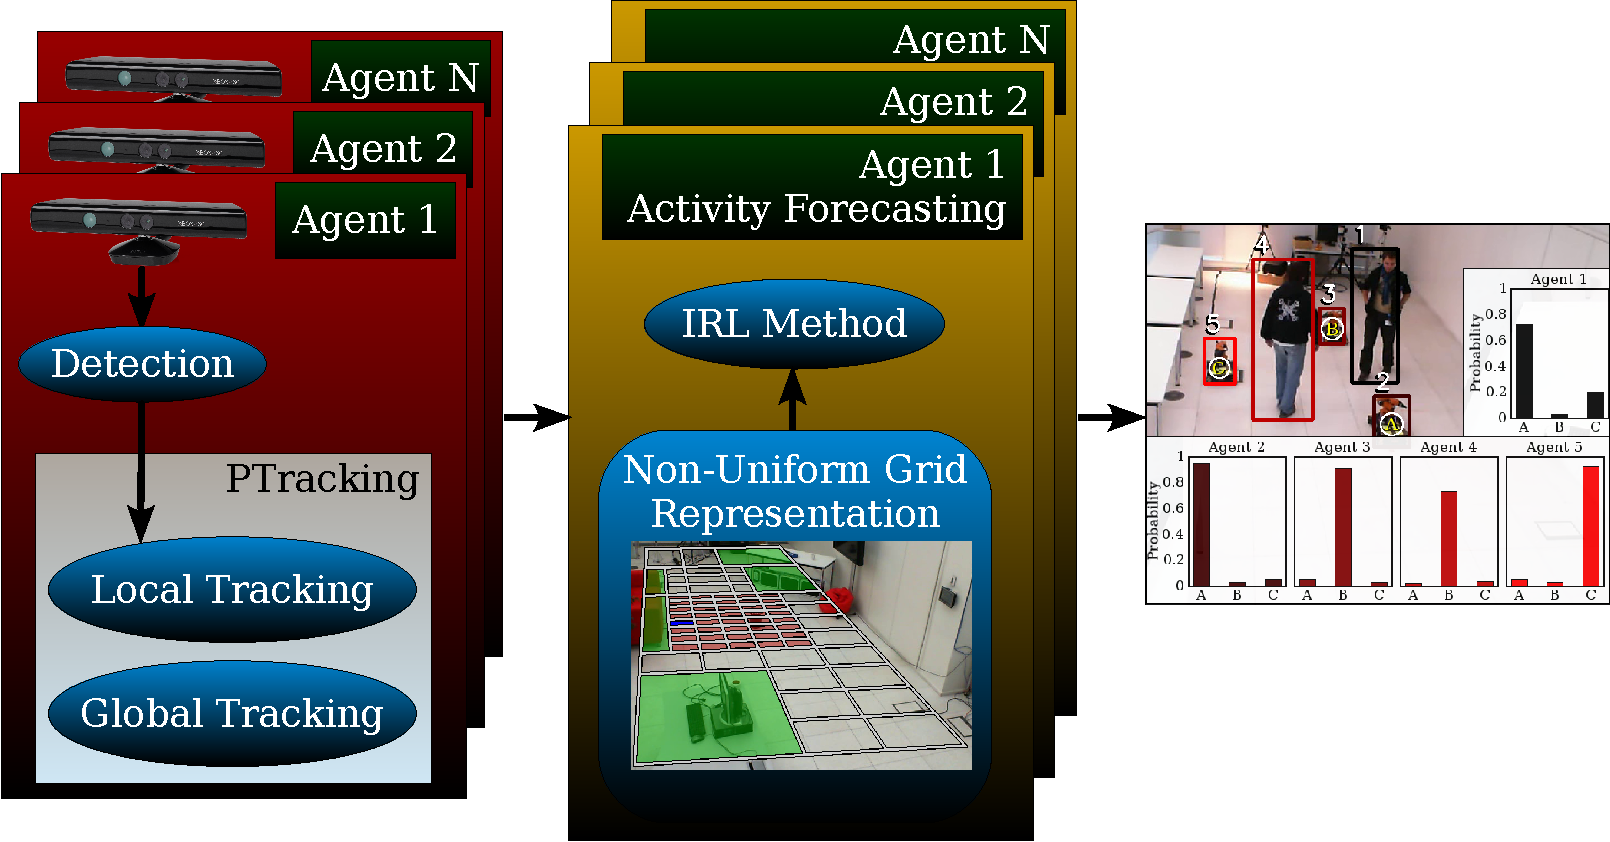
\includegraphics[width=\linewidth]{Figures/Architecture}
		};
	\end{tikzpicture}
\end{frame}

\begin{frame}
	\frametitle{PTracking}
	
	\vspace{0.15cm}
	
	\begin{columns}[T]
		\column{.5\textwidth}
		
		\vspace{0.8cm}
		
		\begin{itemize}
			\item \textbf{Input:} a set of positions of the objects provided by a multi
				  object detection system [4]
			
			\vspace{1.6cm}
			
			\item \textbf{Output:} a set of estimated trajectories of the moving objects
				  over time
		\end{itemize}
		
		\column{.5\textwidth}
		\centering
		
		\begin{tikzpicture}
			\node at (0,0) [draw=black,ultra thick,inner sep=0pt]
			{
				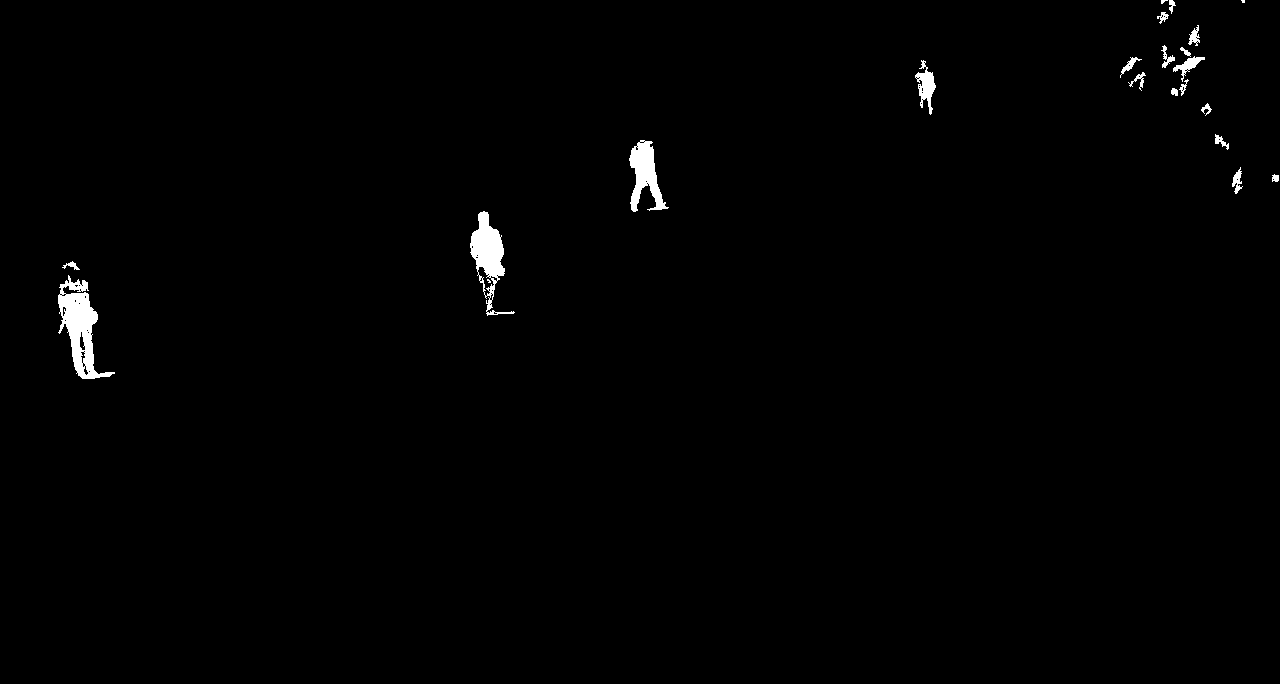
\includegraphics[width=6cm]{Figures/Detection}
			};
			\node at (0,-3.35) [draw=black,ultra thick,inner sep=0pt]
			{
				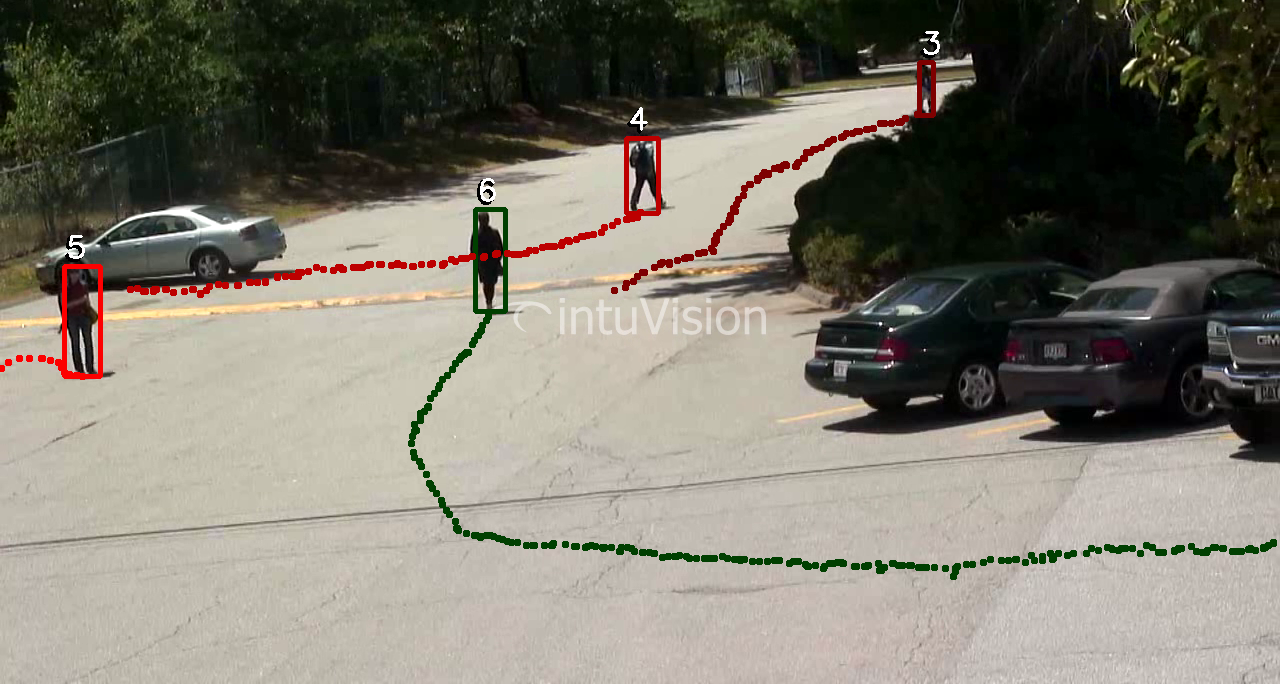
\includegraphics[width=6cm]{Figures/Tracking}
			};
		\end{tikzpicture}
	\end{columns}
	
	\vspace{0.3cm}
	
	\tiny
	
	[4] D. D. Bloisi, L. Iocchi, ``Independent Multimodal Background Subtraction'',
		CompIMAGE, 2012
\end{frame}

\begin{frame}
	\frametitle{PTracking}
	\framesubtitle{Pseudo-code}
	
	\begin{columns}[T]
		\column{.05\textwidth}
		
		\column{.55\textwidth}
		
		\only<1>
		{
			\begin{algorithm}[H]
				\tiny
				\KwIn{perceptions $ z_{s,t} $, local track numbers $ oi_{s,t-1} $, global track numbers $ OI_{s,t-1} $}
				\BlankLine
				\KwData{set of local particles $ \tilde{\xi}_{s,t} $, set of global particles $ \tilde{\xi}_{\mathcal{S'},t} $, local GMM set $ \mathcal{L} $, global GMM set $ \mathcal{G} $}
				\BlankLine
				\KwOut{global estimations $ x_{s,t} = (\boldsymbol{OI}_{s,t},\boldsymbol\Lambda_{s,t},\boldsymbol{M}_{s,t},\boldsymbol\Sigma_{s,t}) $}
				\BlankLine
				\Begin
				{
					\textcolor{darkgreen}{$ \tilde{\xi}_{s,t} \sim \pi_t (x_{s,t} | x_{s,t-1},z_{s,t}) $}
					\BlankLine
					\textcolor{darkgreen}{Re-sample by using the SIR principle}\\
					\BlankLine
					\textcolor{darkgreen}{$ \mathcal{L} = KClusterize(\tilde{\xi}_{s,t}) $}
					\BlankLine
					\textcolor{darkgreen}{$ (\boldsymbol{oi}_{s,t},\boldsymbol\lambda_{s,t},\boldsymbol\mu_{s,t},\boldsymbol\sigma_{s,t}) = DataAssociation(\mathcal{L}, oi_{s,t-1}) $}
					\BlankLine
					\textcolor{darkgreen}{Communicate belief $ (\boldsymbol{oi}_{s,t},\boldsymbol\lambda_{s,t},\boldsymbol\mu_{s,t},\boldsymbol\sigma_{s,t}) $ to other agents}
				}
				\BlankLine
				\Begin
				{
					Collect $ \mathcal{L}_{S'} $ from a subset $ \mathcal{S'} \subseteq \mathcal{S} $ of sensors within a $ \Delta t $
					\BlankLine
					$ \tilde{\xi}_{\mathcal{S'},t} \sim \tilde\pi = \sum_{s \in \mathcal{S'}} \boldsymbol\lambda_{s,t} \, \mathcal{N} (\boldsymbol\mu_{s,t},\boldsymbol\sigma_{s,t}) $
					\BlankLine
					Re-sample by using the SIR principle\\
					\BlankLine
					$ \mathcal{G} = KClusterize(\tilde\xi_{{\mathcal{S'},t}}) $
					\BlankLine
					$ (\boldsymbol{OI}_{s,t},\boldsymbol\Lambda_{s,t},\boldsymbol{M}_{s,t},\boldsymbol\Sigma_{s,t}) = DataAssociation(\mathcal{G},OI_{s,t-1}) $
				}
			\end{algorithm}
			
			\column{.01\textwidth}
			
			\Huge
			\vspace{2.15cm}
			
			\begin{center}
				\textcolor{blue}{$ \Rightarrow $}
			\end{center}
			
			\column{.44\textwidth}
			
			\centering
			
			\begin{tikzpicture}
				\node at (0,0) [draw=black,ultra thick,inner sep=0pt]
				{
					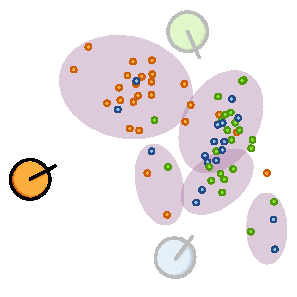
\includegraphics[width=3.3cm]{Figures/Mamot-1}
				};
				\node at (0,-3.5) [draw=black,ultra thick,inner sep=0pt]
				{
					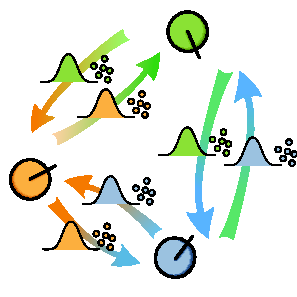
\includegraphics[width=3.3cm]{Figures/Mamot-2}
				};
			\end{tikzpicture}
		}
		
		\only<2->
		{
			\begin{algorithm}[H]
				\tiny
				\KwIn{perceptions $ z_{s,t} $, local track numbers $ oi_{s,t-1} $, global track numbers $ OI_{s,t-1} $}
				\BlankLine
				\KwData{set of local particles $ \tilde{\xi}_{s,t} $, set of global particles $ \tilde{\xi}_{\mathcal{S'},t} $, local GMM set $ \mathcal{L} $, global GMM set $ \mathcal{G} $}
				\BlankLine
				\KwOut{global estimations $ x_{s,t} = (\boldsymbol{OI}_{s,t},\boldsymbol\Lambda_{s,t},\boldsymbol{M}_{s,t},\boldsymbol\Sigma_{s,t}) $}
				\BlankLine
				\Begin
				{
					$ \tilde{\xi}_{s,t} \sim \pi_t (x_{s,t} | x_{s,t-1},z_{s,t}) $
					\BlankLine
					Re-sample by using the SIR principle\\
					\BlankLine
					$ \mathcal{L} = KClusterize(\tilde{\xi}_{s,t}) $
					\BlankLine
					$ (\boldsymbol{oi}_{s,t},\boldsymbol\lambda_{s,t},\boldsymbol\mu_{s,t},\boldsymbol\sigma_{s,t}) = DataAssociation(\mathcal{L}, oi_{s,t-1}) $
					\BlankLine
					Communicate belief $ (\boldsymbol{oi}_{s,t},\boldsymbol\lambda_{s,t},\boldsymbol\mu_{s,t},\boldsymbol\sigma_{s,t}) $ to other agents
				}
				\BlankLine
				\Begin
				{
					\textcolor{lightred}{Collect $ \mathcal{L}_{S'} $ from a subset $ \mathcal{S'} \subseteq \mathcal{S} $ of sensors within a $ \Delta t $}
					\BlankLine
					\textcolor{lightred}{$ \tilde{\xi}_{\mathcal{S'},t} \sim \tilde\pi = \sum_{s \in \mathcal{S'}} \boldsymbol\lambda_{s,t} \, \mathcal{N} (\boldsymbol\mu_{s,t},\boldsymbol\sigma_{s,t}) $}
					\BlankLine
					\textcolor{lightred}{Re-sample by using the SIR principle}\\
					\BlankLine
					\textcolor{lightred}{$ \mathcal{G} = KClusterize(\tilde\xi_{{\mathcal{S'},t}}) $}
					\BlankLine
					\textcolor{lightred}{$ (\boldsymbol{OI}_{s,t},\boldsymbol\Lambda_{s,t},\boldsymbol{M}_{s,t},\boldsymbol\Sigma_{s,t}) = DataAssociation(\mathcal{G},OI_{s,t-1}) $}
				}
			\end{algorithm}
			
			\column{.01\textwidth}
			
			\Huge
			\vspace{2.15cm}
			
			\begin{center}
				\textcolor{blue}{$ \Rightarrow $}
			\end{center}
			
			\column{.44\textwidth}
			
			\centering
			
			\begin{tikzpicture}
				\node at (0,0) [draw=black,ultra thick,inner sep=0pt]
				{
					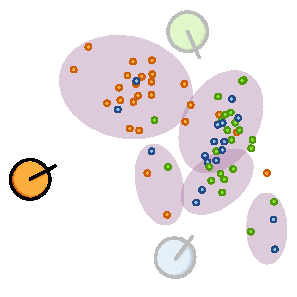
\includegraphics[width=3.3cm]{Figures/Mamot-1}
				};
				\node at (0,-3.5) [draw=black,ultra thick,inner sep=0pt]
				{
					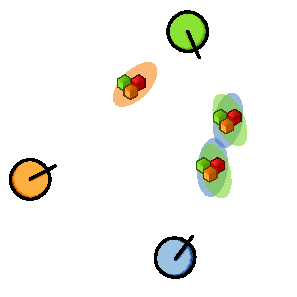
\includegraphics[width=3.3cm]{Figures/Mamot-3}
				};
			\end{tikzpicture}
		}
	\end{columns}
\end{frame}

\begin{frame}
	\frametitle{Activity Forecasting and Anomaly Detection}
	
	\begin{columns}[T]
		\column{.4\textwidth}
		
		\vspace{-0.2cm}
		
		\begin{equation*}
			\hspace{0.3cm}
			\scriptsize
			\begin{array}{ll}
				\min \sum\limits_{i=1}^N -x_i + \lambda (r_i^+ - r_i^-)
				\vspace{-0.35cm} \\ \\
				s.t. \\ \;\;\;\;
				\left \{
					\begin{array}{ll}
						x_i \leq (\mathbf{P}_{a_*} - \mathbf{P}_a)(\mathbf{I} - \gamma
						\mathbf{P}_{a_*})^{-1} \mathbf{R} \\
						\vspace{-0.25cm} \\
						\;\;\;\;\;\;\;\;\;\;\;\;\;\;\;\;\;\;\;\;\;
						\;\;\; \forall \, a \in \mathbf{A}, \; i \in \{ 1, \ldots, N \}
						\vspace{-0.25cm}\\ \\
						x_i \geq 0 \;\;\;\;\;\;\,\,\,\,\;\;\;\,\,\,\,\,\;\,\,\,\,\,\,\,\;\;\;\;\;
						\;\,\,\,\,\, i \in \{ 1, \ldots, N \}
						\vspace{-0.25cm} \\ \\
						r_i = r_i^+ + r_i^- \;\,\,\,\,\,\;\,\,\,\,\,\,\,\;\;\;\;\;
						\;\,\,\,\,\, i \in \{ 1, \ldots, N \}
						\vspace{-0.25cm}
						\\ \\
						| \mathbf{R}_i | \leq R_{max} \;\;\;\;\;\;\;\;\;\;\;\,\,\,\,\;\;\
						\,\,\,\,\,\, i \in \{ 1, \ldots, N \}
					\end{array}
				\right.
				\vspace{0.2cm}
			\end{array}
		\end{equation*}
		
		\tiny
		
		\vspace{-0.8cm}
		
		\begin{tabbing}
			\hspace{0.2cm}
			Adapted formalisation of [Ng \& Russel, 2000]
		\end{tabbing}
		
		\vspace{-1cm}
		
		\column{.15\textwidth}
		
		\centering
		\vspace{1.3cm}
		
		\begin{tabbing}
			\hspace{1.5cm}
			\Huge
			\textcolor{red}{\textbf{+}}
		\end{tabbing}
		
		\column{.45\textwidth}
		\centering
		
		\vspace{0.4cm}
		
		\begin{tikzpicture}
			\node at (0,0) [draw=black,ultra thick,inner sep=0pt]
			{
				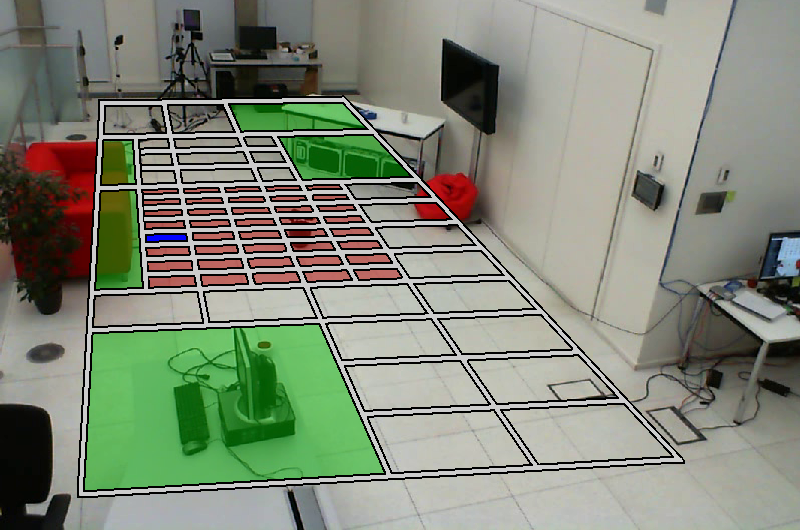
\includegraphics[width=4.8cm]{Figures/RecursiveNonUniformGrids}
			};
		\end{tikzpicture}
	\end{columns}
	
	\vspace{0.2cm}
	
	\begin{columns}[T]
		\column{.35\textwidth}
		
		\vspace{0.3cm}
		
		\begin{tikzpicture}
			\hspace{0.2cm}
			\centering
			\node at (0,0) [draw=white,ultra thick,inner sep=0pt]
			{
				\includegraphics[height=3.2cm]{Figures/IRL-Model}
			};
		\end{tikzpicture}
		
		\column{.2\textwidth}
		
		\centering
		\vspace{1.4cm}
		
		\begin{tabbing}
			\hspace{1.975cm}
			\Huge
			\textcolor{red}{\textbf{$ \Rightarrow $}}
		\end{tabbing}
		
		\column{.45\textwidth}
		\centering
		
		\vspace{0.3cm}
		
		\begin{tikzpicture}
			\node at (0,0) [draw=black,ultra thick,inner sep=0pt]
			{
				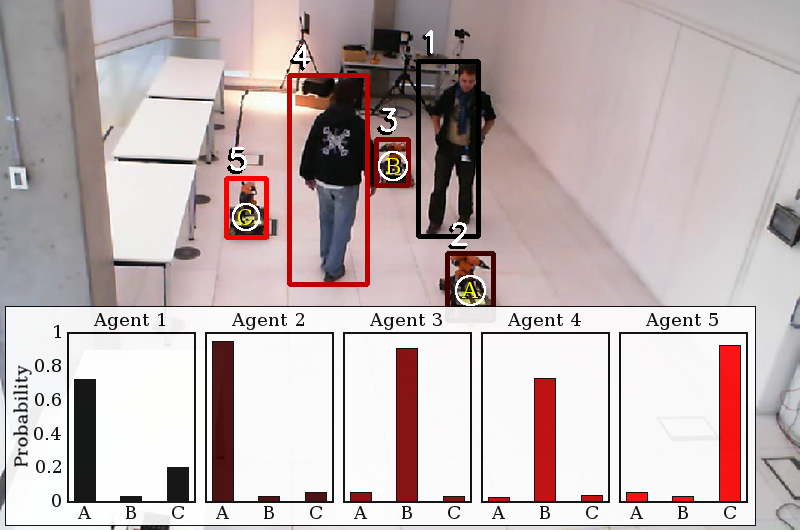
\includegraphics[width=4.8cm]{Figures/Motivation}
			};
		\end{tikzpicture}
	\end{columns}
	
	\begin{columns}[T]
		\column{\textwidth}
		
		\centering
		\vspace{-3.1cm}
		\hspace{-1cm}
		\Huge
		\begin{rotate}{-45}
			
			\textcolor{blue}{\textbf{$ \Downarrow $}}
		\end{rotate}	
	\end{columns}
\end{frame}

\begin{frame}
	\frametitle{Activity Forecasting}
	
	\Large
	
	\vspace{1.2cm}
	
	The output of the optimisation process is a \textbf{set of $ \mathbf{G}^1 $ reward
	function models}, one for each goal, $ \mathbf{\mathcal{M}_s^G} $ per agent $ s $. \\
	
	\vspace{0.4cm}
	
	This allows us to generate a policy $ \pi_s^{G_i} $ for each goal $ G_i \in G $ per
	agent $ s $. \\
	
	\vspace{2cm}
	
	\normalsize
	
	1. Goals can be \emph{statically} chosen or \emph{generated} by analysing tracking data
\end{frame}

\begin{frame}
	\frametitle{Activity Forecasting}
	\framesubtitle{Observed Trajectory Extraction}
	
	\Large
	
	\vspace{0.4cm}
	
	We gather object estimates from PTracking considering an arbitrary temporal window. \\
	
	\vspace{0.4cm}
	
	Having acquired a set of trajectories $ \mathcal{U} $, we \textbf{ground} each
	trajectory $ u \in \mathcal{U} $ in every policy $ \pi_s^G $. \\
\end{frame}

\begin{frame}
	\frametitle{Activity Forecasting}
	\framesubtitle{Policy Comparison}
	
	\Large
	
	\vspace{0.1cm}
	
	We get the best fitting policy by \textbf{comparing} the target trajectory against a
	set of trajectories drawn from potential optimal policies. \\
	
	\vspace{0.4cm}
	
	We use a combination of \emph{Fr\'echet distance} and \emph{cosine similarity}, to
	allow for the possibility that the target trajectory is merely a fragment of the
	overall optimal policy. \\
\end{frame}

\begin{frame}
	\frametitle{Activity Forecasting}
	\framesubtitle{Goal Prediction}
	
	\large
	
	\vspace{0.4cm}
	
	We are finally able to \textbf{predict in real-time} the goal toward which each moving
	object is likely to be headed, by executing the policy that best matches the movement
	pattern of every object. \\
	
	\begin{center}
		\begin{tikzpicture}
			\node at (0,0) [draw=white,ultra thick,inner sep=0pt]
			{
				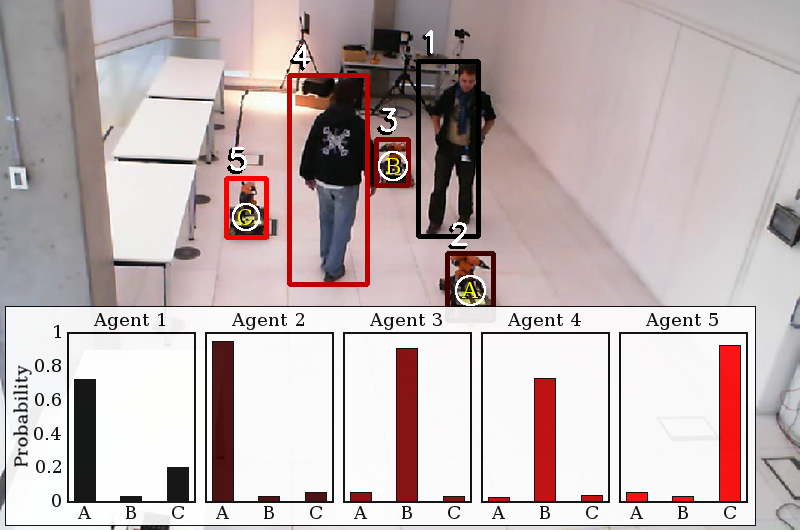
\includegraphics[width=0.62\linewidth]{Figures/Motivation}
			};
		\end{tikzpicture}
	\end{center}
\end{frame}

\begin{frame}
	\frametitle{Anomaly Detection}
	
	\Large
	
	\vspace{0.3cm}
	
	It could happen that a trajectory $ u \in \mathcal{U} $ does not match any model:
	
	\begin{itemize}
		\item a trajectory fragment $ u $ is \textbf{anomalous} and refers to a
			  \emph{suspicious activity pattern}
		\item environment has changed leading to new types of motion
			  \vspace{-0.1cm}
			  \begin{tabbing}
				  \hspace{0.3cm}
				  \large
				  $ \leadsto $ \emph{can be recognised by analysing the foreground model}
			  \end{tabbing}
	\end{itemize}
\end{frame}
